\documentclass[tikz,border=2pt]{standalone}
\begin{document}
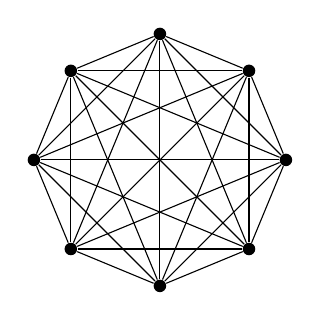
\begin{tikzpicture}[vertex/.style={circle,fill,inner sep=1.6pt}]
    \foreach \i in {1,...,8}{
        \node[vertex] (v\i) at ({90-(\i-1)*45}:1.6) {};
    }
    \foreach \i in {1,...,8}{
        \foreach \j in {1,...,8}{
            \ifnum\i<\j
                \draw (v\i) -- (v\j);
            \fi
        }
    }
\end{tikzpicture}
\end{document}
